%%____________________________________________________________________________||
\section{Interpretation in Dark Matter models}
\label{sec:darkmatter}

In Run~1, the \alphat analysis was used to interpret models with supersymmetry and their simplified models. In Run~2, significant effort has been invested to extended the analysis strategy to include searches for the production of dark matter (DM) in  proton-proton collisions, namely the asymmetric and monojet jet categories.


%The generic signature of dark matter pair production in colliders is missing transverse momentum from the  dark matter and energetic visible particles that are used to trigger the event. First analyses using this final state  used contact operators~\cite{Goodman:2010ku} with couplings between dark matter and quarks. The resulting ``monojet'' final state consists of one or two hard jets plus large missing transverse momentum from the dark matter. Experimental limits using monojet final states have been published using 7 and 8 TeV LHC data \cite{Chatrchyan:2012me,ATLAS:2012ky} for a variety of operators.
%However, lack of predictive information and severe validity constraints have lead to extended and improved minimal simplified dark matter models (MSDM) that allow to relate the different experimental signatures in a relatively model-independent way~\cite{Buchmueller:2014yoa}. 

%In addition, similar final states with the form $\chi \bar \chi + X$, where $\chi$ is the dark matter particle
%and $X$ can be a photon, jet, or other particle, have been studied in the context of effective operators These additional particles are initial state radiation (ISR) 
%radiated off from the interacting partons. (e.g. \cite{Goodman:2010yf,Fox:2011pm,Petriello:2008pu,Fox:2011fx}).


%Previous CMS analyses performed the search for new physics in the monojet final state, as detailed in References~\cite{Aad:2011xw, ATLAS:2012ky} using up to $4.7\,\fbi$ 
%of data with proton-proton collision at a center-of-mass energy of $\sqrt{s}=7\,\tev$. A conference note~\cite{ATLAS-CONF-2012-147} using 8$\,\tev$ data has also been published, 
%based on half of the 2012 dataset. 


%The present document also describes the planned analysis of WIMP pair production in association with light and heavy quarks using the upcoming 13~TeV data set corresponding. 
%Hadronic final states of the form $\chi \bar \chi + X$, where $\chi$ is the dark matter particle and $X$ can be one or several jets have been studied in the context of effective operators. These jets are either directly produced due in the interaction between SM and DM or are initial state radiation (ISR)  radiated off from the interacting partons (e.g. \cite{Goodman:2010yf,Fox:2011pm,Petriello:2008pu,Fox:2011fx}). As detailed in Ref.~\cite{Lin:2013sca, Artoni:2013zba} particular the use of heavy quarks, namely $b$- and top quarks take advantage of quark-mass dependency of scalar couplings. The quark mass dependency comes from minimal flavor violation assumptions. Further advantages gained by the use of third generation quarks is to extend the analysis to larger jet multiplicities and therefore larger signal acceptance compared to the monojet analysis. Thus accessing a unique and orthogonal phase space. 


%This analysis will also set strongest constraints for low mass dark matter, and the strongest collider constraints across a wide range of masses. We will also start to probe excesses observed in direct detection experiment at energies of about 10 GeV in the DAMA (2008), CoGent (2010/11), CREST-II (2012) and CDMS (2013) experiments but also by the Fermi-LAT (2013) satellite indicating a DM particle of about 50 GeV mass. We expect to place stringent constraints on this phase space in the near future with the $13$~TeV run.




%\subsection{Simplified Models}


The primary simplified models for Dirac fermion DM studied and recommended by the ATLAS-CMS DM Forum for early LHC Run-2 searches are comprised of spin-0 and spin-1 mediators using $s$-channel and $t$-channel models.We consider the case of a DM particle $\chi$ of mass $m_{\chi}$ that is a Dirac fermion and where the production proceeds via the exchange
of a spin-1 mediator $\Phi$ of mass $m_{\Phi}$ in the $s$-channel. Two models with vector (V) and axial-vector (AV) couplings are considered. The coupling to the standard model
$g_{\textrm SM}$ is assumed to be universal for all quark families and $g_{\textrm DM}$ is the coupling to the dark matter particles. Assuming that not additional visible or invisible particles contribute to the decay we use the minimal width determined by the choice of $g_{\textrm SM}$ and $g_{\textrm DM}$ as shown in Fig.~\ref{fig:feynman}.

\begin{figure}[h!]
  \centering
  \subfigure{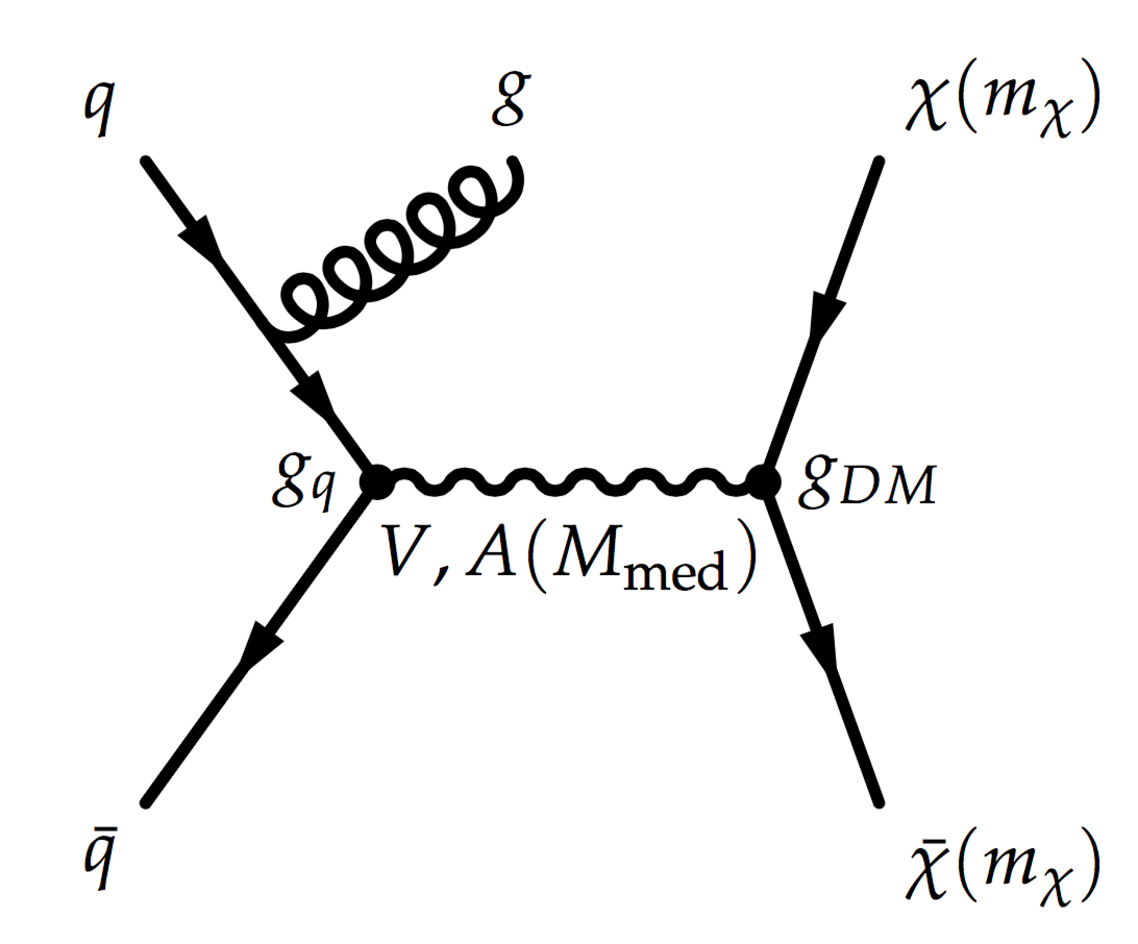
\includegraphics[width=0.5\textwidth]{figures/DMplots/feynman_light_jet.pdf}}
  \caption{Representative Feynman diagram showing the pair production of Dark Matter particles in association with a parton from the initial state via a vector or axial-vector mediator. The cross section and kinematics depend upon the mediator and Dark Matter masses, and the mediator couplings to Dark Matter and quarks respectively: ($m_{\Phi} ,\ m_\textrm{DM} ,\, g_{\textrm DM} ,\, g_{\textrm SM})$. \cite{Abercrombie:2015wmb}}
  \label{fig:feynman}
\end{figure}

$M_{\Phi}$ grid points are chosen, roughly equidistant in a logarithmic scale: 10,~20, 50, 100, 200, 300, 500, 1000 and 2000 GeV. In the  threshold regime $M_{\Phi} = 2 \times m_{\chi}$, the $ m_{\chi}$ grid points are taken at approximately $M_{\Phi}/2$. Points on the on-shell diagonal are always chosen to be
5 GeV away from the threshold, to avoid numerical instabilities in the event generation. 


\begin{table}[h!]
\centering
\begin{tabular}{l|llllllllll}\hline \hline
$m_\textrm{DM}$  & \multicolumn{10}{c}{$m_\Phi$}                                   \\ \hline
1    & 10 & 20 & 50 & 100 & 200 & 300 & 500 & 1000 & 2000 & 10000 \\
10   & 10 & 15 & 50 & 100 &     &     &     &      &      & 10000 \\
50   & 10 &    & 50 & 95  & 200 & 300 &     &      &      & 10000 \\
150  & 10 &    &    &     & 200 & 295 & 500 & 1000 &      & 10000 \\
500  & 10 &    &    &     &     &     & 500 & 995  &      & 10000 \\
1000 & 10 &    &    &     &     &     &     & 1000 & 1995 & 10000\\ \hline
\hline
\end{tabular}
\caption{Dark matter and mediator mass grid analysed. The parameter space follows the DM Forum recommendations~\cite{Abercrombie:2015wmb}}
\label{tab:DMgrid}
\end{table}

\subsection{Light Jet Models}

\begin{table}[]
\centering
\small
\begin{tabular}{lll||lll}
\hline
Dataset name        & Cross section [pb]  & Events    & Dataset name  & Cross section [pb]  & events           \\\hline
$m_\phi=$10000 $m_\textrm{DM}=$1000 & 7.26E-09     & 50000                  &  $m_\phi=$200 $m_\textrm{DM}=$10     & 2.45E+01     & 50000                  \\ 
$m_\phi=$10000 $m_\textrm{DM}=$100  & 1.12E-06     & 50000                  &  $m_\phi=$200 $m_\textrm{DM}=$150    & 3.03E-01     & 50000                  \\ 
$m_\phi=$10000 $m_\textrm{DM}=$10   & 1.31E-06     & 50000                  &  $m_\phi=$200 $m_\textrm{DM}=$1      & 2.45E+01     & 50000                  \\ 
$m_\phi=$10000 $m_\textrm{DM}=$150  & 9.14E-07     & 50000                  &  $m_\phi=$200 $m_\textrm{DM}=$50     & 2.44E+01     & 50000                  \\ 
$m_\phi=$10000 $m_\textrm{DM}=$1    & 1.29E-06     & 50000                  &  $m_\phi=$20 $m_\textrm{DM}=$10      & 8.70E+00     & 50000                  \\ 
$m_\phi=$10000 $m_\textrm{DM}=$500  & 9.05E-08     & 50000                  &  $m_\phi=$20 $m_\textrm{DM}=$1       & 2.66E+02     & 50000                  \\ 
$m_\phi=$10000 $m_\textrm{DM}=$50   & 1.25E-06     & 50000                  &  $m_\phi=$300 $m_\textrm{DM}=$100    & 1.88E+01     & 50000                  \\ 
$m_\phi=$1000 $m_\textrm{DM}=$1000  & 2.69E-06     & 50000                  &  $m_\phi=$300 $m_\textrm{DM}=$10     & 1.89E+01     & 50000                  \\ 
$m_\phi=$1000 $m_\textrm{DM}=$100   & 7.68E-02     & 50000                  &  $m_\phi=$300 $m_\textrm{DM}=$150    & 2.11E+00     & 50000                  \\ 
$m_\phi=$1000 $m_\textrm{DM}=$10    & 7.99E-02     & 50000                  &  $m_\phi=$300 $m_\textrm{DM}=$1      & 1.89E+01     & 50000                  \\ 
$m_\phi=$1000 $m_\textrm{DM}=$150   & 7.29E-02     & 50000                  &  $m_\phi=$300 $m_\textrm{DM}=$50     & 1.89E+01     & 50000                  \\ 
$m_\phi=$1000 $m_\textrm{DM}=$1     & 7.99E-02     & 50000                  &  $m_\phi=$5000 $m_\textrm{DM}=$1000  & 2.56E-07     & 50000                  \\ 
$m_\phi=$1000 $m_\textrm{DM}=$500   & 9.34E-03     & 50000                  &  $m_\phi=$5000 $m_\textrm{DM}=$100   & 1.88E-05     & 50000                  \\ 
$m_\phi=$1000 $m_\textrm{DM}=$50    & 7.91E-02     & 50000                  &  $m_\phi=$5000 $m_\textrm{DM}=$10    & 2.16E-05     & 50000                  \\ 
$m_\phi=$100 $m_\textrm{DM}=$100    & 4.29E-01     & 50000                  &  $m_\phi=$5000 $m_\textrm{DM}=$150   & 1.55E-05     & 50000                  \\ 
$m_\phi=$100 $m_\textrm{DM}=$10     & 5.88E+01     & 50000                  &  $m_\phi=$5000 $m_\textrm{DM}=$1     & 2.16E-05     & 50000                  \\ 
$m_\phi=$100 $m_\textrm{DM}=$1      & 5.88E+01     & 50000                  &  $m_\phi=$5000 $m_\textrm{DM}=$500   & 1.80E-06     & 50000                  \\ 
$m_\phi=$100 $m_\textrm{DM}=$50     & 3.36E+00     & 50000                  &  $m_\phi=$5000 $m_\textrm{DM}=$50    & 2.09E-05     & 50000                  \\ 
$m_\phi=$10 $m_\textrm{DM}=$10      & 6.64E+00     & 50000                  &  $m_\phi=$500 $m_\textrm{DM}=$100    & 3.00E+00     & 50000                  \\ 
$m_\phi=$10 $m_\textrm{DM}=$1       & 3.68E+02     & 50000                  &  $m_\phi=$500 $m_\textrm{DM}=$10     & 3.17E+00     & 50000                  \\ 
$m_\phi=$2000 $m_\textrm{DM}=$1000  & 7.83E-05     & 50000                  &  $m_\phi=$500 $m_\textrm{DM}=$150    & 2.72E+00     & 50000                  \\ 
$m_\phi=$2000 $m_\textrm{DM}=$100   & 1.46E-03     & 50000                  &  $m_\phi=$500 $m_\textrm{DM}=$1      & 3.17E+00     & 50000                  \\ 
$m_\phi=$2000 $m_\textrm{DM}=$10    & 1.58E-03     & 50000                  &  $m_\phi=$500 $m_\textrm{DM}=$500    & 4.11E-04     & 50000                  \\ 
$m_\phi=$2000 $m_\textrm{DM}=$150   & 1.32E-03     & 50000                  &  $m_\phi=$500 $m_\textrm{DM}=$50     & 3.13E+00     & 50000                  \\ 
$m_\phi=$2000 $m_\textrm{DM}=$1     & 1.58E-03     & 50000                  &  $m_\phi=$50 $m_\textrm{DM}=$10      & 1.28E+02     & 50000                  \\ 
$m_\phi=$2000 $m_\textrm{DM}=$500   & 6.10E-04     & 50000                  &  $m_\phi=$50 $m_\textrm{DM}=$1       & 1.28E+02     & 50000                  \\ 
$m_\phi=$2000 $m_\textrm{DM}=$50    & 1.55E-03     & 50000                  &  $m_\phi=$50 $m_\textrm{DM}=$50      & 1.04E+00     & 50000                  \\
$m_\phi=$200 $m_\textrm{DM}=$100    & 2.10E+00     & 50000                  & \\\hline
\end{tabular}
\caption{Simplified DM samples for light jets and pseudoscalar DM couplings. All samples are generated for $\sqrt{s}=13~$TeV and $g_\textrm{SM}=g_\textrm{DM}=1$.}
\label{tab:samples_ps}
\end{table}




\begin{table}[]
\centering
\small
\begin{tabular}{lll||lll}
\hline
Dataset name        & Cross section [pb]  & Events    & Dataset name  & Cross section [pb]  & events           \\\hline
$m_\phi=$10000 $m_\textrm{DM}=$1000       & 2.39E-09     & 50000                  & $m_\phi=$200 $m_\textrm{DM}=$10           & 9.94E+00     & 50000                  \\ 
$m_\phi=$10000 $m_\textrm{DM}=$100        & 5.50E-07     & 50000                  & $m_\phi=$200 $m_\textrm{DM}=$150          & 4.67E-02     & 50000                  \\ 
$m_\phi=$10000 $m_\textrm{DM}=$10         & 6.69E-07     & 50000                  & $m_\phi=$200 $m_\textrm{DM}=$1            & 9.94E+00     & 50000                  \\ 
$m_\phi=$10000 $m_\textrm{DM}=$150        & 4.01E-07     & 50000                  & $m_\phi=$200 $m_\textrm{DM}=$50           & 9.96E+00     & 50000                  \\ 
$m_\phi=$10000 $m_\textrm{DM}=$1          & 6.71E-07     & 50000                  & $m_\phi=$20 $m_\textrm{DM}=$10            & 2.40E+00     & 50000                  \\ 
$m_\phi=$10000 $m_\textrm{DM}=$500        & 3.67E-08     & 50000                  & $m_\phi=$20 $m_\textrm{DM}=$1             & 1.18E+02     & 50000                  \\ 
$m_\phi=$10000 $m_\textrm{DM}=$50         & 6.24E-07     & 50000                  & $m_\phi=$300 $m_\textrm{DM}=$100          & 6.23E+00     & 50000                  \\ 
$m_\phi=$1000 $m_\textrm{DM}=$1000        & 5.65E-07     & 50000                  & $m_\phi=$300 $m_\textrm{DM}=$10           & 6.21E+00     & 50000                  \\ 
$m_\phi=$1000 $m_\textrm{DM}=$100         & 5.63E-02     & 50000                  & $m_\phi=$300 $m_\textrm{DM}=$150          & 1.33E-01     & 50000                  \\ 
$m_\phi=$1000 $m_\textrm{DM}=$10          & 6.02E-02     & 50000                  & $m_\phi=$300 $m_\textrm{DM}=$1            & 6.21E+00     & 50000                  \\ 
$m_\phi=$1000 $m_\textrm{DM}=$150         & 5.19E-02     & 50000                  & $m_\phi=$300 $m_\textrm{DM}=$50           & 6.21E+00     & 50000                  \\ 
$m_\phi=$1000 $m_\textrm{DM}=$1           & 6.03E-02     & 50000                  & $m_\phi=$5000 $m_\textrm{DM}=$1000        & 1.17E-07     & 50000                  \\ 
$m_\phi=$1000 $m_\textrm{DM}=$500         & 8.73E-04     & 50000                  & $m_\phi=$5000 $m_\textrm{DM}=$100         & 8.99E-06     & 50000                  \\ 
$m_\phi=$1000 $m_\textrm{DM}=$50          & 5.92E-02     & 50000                  & $m_\phi=$5000 $m_\textrm{DM}=$10          & 1.14E-05     & 50000                  \\ 
$m_\phi=$100 $m_\textrm{DM}=$100          & 8.96E-02     & 50000                  & $m_\phi=$5000 $m_\textrm{DM}=$150         & 6.93E-06     & 50000                  \\ 
$m_\phi=$100 $m_\textrm{DM}=$10           & 2.56E+01     & 50000                  & $m_\phi=$5000 $m_\textrm{DM}=$1           & 1.14E-05     & 50000                  \\ 
$m_\phi=$100 $m_\textrm{DM}=$1            & 2.56E+01     & 50000                  & $m_\phi=$5000 $m_\textrm{DM}=$500         & 8.06E-07     & 50000                  \\ 
$m_\phi=$100 $m_\textrm{DM}=$50           & 4.99E-01     & 50000                  & $m_\phi=$5000 $m_\textrm{DM}=$50          & 1.07E-05     & 50000                  \\ 
$m_\phi=$10 $m_\textrm{DM}=$10            & 2.02E+00     & 50000                  & $m_\phi=$500 $m_\textrm{DM}=$100          & 1.89E+00     & 50000                  \\ 
$m_\phi=$10 $m_\textrm{DM}=$1             & 1.63E+02     & 50000                  & $m_\phi=$500 $m_\textrm{DM}=$10           & 2.10E+00     & 50000                  \\ 
$m_\phi=$2000 $m_\textrm{DM}=$1000        & 6.85E-06     & 50000                  & $m_\phi=$500 $m_\textrm{DM}=$150          & 1.56E+00     & 50000                  \\ 
$m_\phi=$2000 $m_\textrm{DM}=$100         & 9.44E-04     & 50000                  & $m_\phi=$500 $m_\textrm{DM}=$1            & 2.10E+00     & 50000                  \\ 
$m_\phi=$2000 $m_\textrm{DM}=$10          & 1.05E-03     & 50000                  & $m_\phi=$500 $m_\textrm{DM}=$500          & 9.75E-05     & 50000                  \\ 
$m_\phi=$2000 $m_\textrm{DM}=$150         & 8.44E-04     & 50000                  & $m_\phi=$500 $m_\textrm{DM}=$50           & 2.05E+00     & 50000                  \\ 
$m_\phi=$2000 $m_\textrm{DM}=$1           & 1.06E-03     & 50000                  & $m_\phi=$50 $m_\textrm{DM}=$10            & 5.69E+01     & 50000                  \\ 
$m_\phi=$2000 $m_\textrm{DM}=$500         & 3.94E-04     & 50000                  & $m_\phi=$50 $m_\textrm{DM}=$1             & 5.67E+01     & 50000                  \\ 
$m_\phi=$2000 $m_\textrm{DM}=$50          & 1.02E-03     & 50000                  & $m_\phi=$50 $m_\textrm{DM}=$50            & 2.61E-01     & 50000                   \\  
$m_\phi=$200 $m_\textrm{DM}=$100          & 2.15E-01     & 50000                  \\\hline
\end{tabular}
\caption{Simplified DM samples for light jets and scalar DM couplings. All samples are generated for $\sqrt{s}=13~$TeV and $g_\textrm{SM}=g_\textrm{DM}=1$.}
\label{tab:samples_s}
\end{table}



\begin{table}[]
\centering
\small
\begin{tabular}{lll||lll}
\hline
Dataset name        & Cross section [pb]  & Events    & Dataset name  & Cross section [pb]  & events           \\\hline
$m_\phi=$10000 $m_\textrm{DM}=$1000  & 3.422E-06 & 50000 & $m_\phi=$2000 $m_\textrm{DM}=$100    & 4.050E-01 & 50000 \\
$m_\phi=$10000 $m_\textrm{DM}=$100   & 5.566E-05 & 50000 & $m_\phi=$2000 $m_\textrm{DM}=$10     & 4.210E-01 & 50000 \\
$m_\phi=$10000 $m_\textrm{DM}=$10    & 7.410E-05 & 50000 & $m_\phi=$2000 $m_\textrm{DM}=$150    & 3.945E-01 & 50000 \\
$m_\phi=$10000 $m_\textrm{DM}=$150   & 4.702E-05 & 50000 & $m_\phi=$2000 $m_\textrm{DM}=$1      & 4.215E-01 & 50000 \\
$m_\phi=$10000 $m_\textrm{DM}=$1     & 7.478E-05 & 50000 & $m_\phi=$2000 $m_\textrm{DM}=$500    & 2.887E-01 & 50000 \\
$m_\phi=$10000 $m_\textrm{DM}=$500   & 1.543E-05 & 50000 & $m_\phi=$2000 $m_\textrm{DM}=$50     & 4.148E-01 & 50000 \\
$m_\phi=$10000 $m_\textrm{DM}=$50    & 6.588E-05 & 50000 & $m_\phi=$200 $m_\textrm{DM}=$10      & 2.021E+03 & 50000 \\
$m_\phi=$1000 $m_\textrm{DM}=$100    & 8.495E+00 & 50000 & $m_\phi=$200 $m_\textrm{DM}=$150     & 2.547E+00 & 50000 \\
$m_\phi=$1000 $m_\textrm{DM}=$10     & 8.987E+00 & 50000 & $m_\phi=$200 $m_\textrm{DM}=$1       & 2.041E+03 & 50000 \\
$m_\phi=$1000 $m_\textrm{DM}=$150    & 8.028E+00 & 50000 & $m_\phi=$200 $m_\textrm{DM}=$50      & 1.584E+03 & 50000 \\
$m_\phi=$1000 $m_\textrm{DM}=$1      & 8.999E+00 & 50000 & $m_\phi=$20 $m_\textrm{DM}=$10       & 4.876E+03 & 50000 \\
$m_\phi=$1000 $m_\textrm{DM}=$500    & 1.308E-01 & 50000 & $m_\phi=$300 $m_\textrm{DM}=$100     & 3.493E+02 & 50000 \\
$m_\phi=$1000 $m_\textrm{DM}=$50     & 8.828E+00 & 50000 & $m_\phi=$300 $m_\textrm{DM}=$10      & 6.030E+02 & 50000 \\
$m_\phi=$100 $m_\textrm{DM}=$100     & 7.719E+00 & 50000 & $m_\phi=$300 $m_\textrm{DM}=$150     & 8.746E+00 & 50000 \\
$m_\phi=$100 $m_\textrm{DM}=$10      & 1.334E+04 & 50000 & $m_\phi=$300 $m_\textrm{DM}=$1       & 6.061E+02 & 50000 \\
$m_\phi=$100 $m_\textrm{DM}=$1       & 1.381E+04 & 50000 & $m_\phi=$500 $m_\textrm{DM}=$100     & 9.563E+01 & 50000 \\
$m_\phi=$100 $m_\textrm{DM}=$50      & 1.735E+02 & 50000 & $m_\phi=$500 $m_\textrm{DM}=$10      & 1.130E+02 & 50000 \\
$m_\phi=$ $m_\textrm{DM}=$1000     & 3.426E-04 & 50000 & $m_\phi=$500 $m_\textrm{DM}=$150     & 7.361E+01 & 50000 \\
$m_\phi=$ $m_\textrm{DM}=$100      & 6.220E+00 & 50000 & $m_\phi=$500 $m_\textrm{DM}=$1       & 1.133E+02 & 50000 \\
$m_\phi=$ $m_\textrm{DM}=$10       & 3.656E+03 & 50000 & $m_\phi=$500 $m_\textrm{DM}=$500     & 1.920E-02 & 50000 \\
$m_\phi=$ $m_\textrm{DM}=$1        & 1.786E+06 & 50000 & $m_\phi=$500 $m_\textrm{DM}=$50      & 1.083E+02 & 50000 \\
$m_\phi=$ $m_\textrm{DM}=$500      & 1.463E-02 & 50000 & $m_\phi=$ $m_\textrm{DM}=$10       & 6.601E+04 & 50000 \\
$m_\phi=$ $m_\textrm{DM}=$50       & 5.115E+01 & 50000 & $m_\phi=$ $m_\textrm{DM}=$1        & 7.598E+04 & 50000 \\
$m_\phi=$2000 $m_\textrm{DM}=$1000   & 4.768E-03 & 50000 & Mchi-50 $m_\textrm{DM}=$50       & 6.231E+01 & 50000 \\
\hline
\end{tabular}
\caption{Simplified DM samples for light jets and axial DM couplings. All samples are generated for $\sqrt{s}=13~$TeV and $g_\textrm{SM}=0.25$, $g_\textrm{DM}=1$.}
\label{tab:samples_a}
\end{table}




We consider four simplified models resulting in final states dominated by light quarks ($u,~d,~c,~s$) production. These models probe the axial-vector (A), vector (V), scalar (S) and pseudo-scalar (P) coupling of the mediator between dark matter and standard model particles. Currently the couplings constants $g_\textrm{DM}$ and $g_\textrm{SM}$ are assumed to be one. This document will be updated to reflect a recent recommendation of $g_\textrm{SM}=0.25$

Assuming 3~fb$^{-1}$ of data we list the expected efficiency and signal yield - divided into nominal and asymmetric selection - in Tables~\ref{tab:dm_A_g1_3fb}-\ref{tab:dm_P_g1_3fb}.

\begin{table}[h!]
\small
\centering
\begin{tabular}{lllllll}
\hline
$m_\textrm{DM}$ & $m_\Phi$  & $\sigma$ [pb] & Sum Evts       & Evts Sym. Bin & Evts Asym. Bin & Eff  [\%]   \\\hline
1000 & 10000 & 3.68E-06 & 0        & 0        & 0        & 4.72 \\
\hline
\hline
\end{tabular}
\caption{Selected axial-vector samples. Given are production cross section, event yields for 3~fb$^{-1 }$ for the various selections and the overall selection efficiency for $g_\textrm{DM}=g_\textrm{SM}=1$}
\label{tab:dm_A_g1_3fb}
\end{table}


\begin{table}[]
\small
\centering
\begin{tabular}{llllll}
$m_\phi$  &  $m_\chi$   &  $\sigma$ [pb] &   yield &  efficiency \\\hline
10    & 1    & 1.94E+07 & 189144.47 & 0    & -1       \\
10    & 10   & 5.17E+04 & 7565.37   & 0    & 0.01     \\
20    & 1    & 3.82E+06 & 65192.5   & 0    & 0        \\
20    & 10   & 8.58E+04 & 3176.59   & 0    & 0.06     \\
50    & 1    & 3.96E+05 & 108876.41 & 0.01 & 0        \\
50    & 50   & 6.32E+02 & 2720.29   & 0.14 & 0.07     \\
200   & 1    & 6.90E+03 & 44656.96  & 0.22 & 0.01     \\
200   & 10   & 6.95E+03 & 40344.29  & 0.19 & 0.01     \\
200   & 50   & 7.19E+03 & 43444.15  & 0.2  & 0.01     \\
200   & 150  & 2.67E+01 & 531.82    & 0.67 & 0.62     \\
300   & 10   & 2.14E+03 & 26353.67  & 0.41 & 0.01     \\
300   & 50   & 1.97E+03 & 24278.81  & 0.41 & 0.01     \\
300   & 100  & 1.93E+03 & 23443.22  & 0.4  & 0.01     \\
300   & 150  & 2.63E+02 & 3654.05   & 0.46 & 0.08     \\
500   & 1    & 3.25E+02 & 8555.77   & 0.88 & 0.04     \\
500   & 10   & 3.48E+02 & 8040.21   & 0.77 & 0.04     \\
500   & 50   & 3.43E+02 & 8049.56   & 0.78 & 0.04     \\
500   & 100  & 3.42E+02 & 7788.44   & 0.76 & 0.04     \\
500   & 150  & 3.28E+02 & 7872.85   & 0.8  & 0.04     \\
500   & 500  & 1.97E-01 & 10.29     & 1.74 & 29.89    \\
1000  & 100  & 2.73E+01 & 1102.79   & 1.35 & 0.3      \\
1000  & 150  & 2.62E+01 & 1122.29   & 1.43 & 0.29     \\
1000  & 1000 & 5.93E-03 & 0.42      & 2.37 & 708.47   \\
10000 & 50   & 2.08E-04 & 0.01      & 1.1  & 47027.64 \\
10000 & 100  & 1.97E-04 & 0.01      & 1.38 & 37658.28 \\
10000 & 150  & 1.74E-04 & 0.01      & 1.56 & 37189.41 \\
10000 & 500  & 7.68E-05 & 0         & 2.07 & 64344.23 \\\hline
\end{tabular}
\caption{Cross section, event yield and efficiencies and for light jets DM samples with vector interactions scaled to 3~fb$^{-1 }$}
\label{tab:dm_V_g1_3fb}
\end{table}




\clearpage
\subsubsection{Scalar and Pseudoscalar Models} \label{sec:dm_pscalar}

\begin{table}[h!]
\small
\centering
\begin{tabular}{lllllll}
\hline
$m_\textrm{DM}$ & $m_\Phi$ & $\sigma$ [pb] & Sum Evts       & Evts Sym. Bin & Evts Asym. Bin & Eff  [\%]   \\\hline
1000  &  10000 & 1.74E-09 & 0      & 0      & 0      & 8.18 \\

\hline
\end{tabular}
\caption{Selected scalar samples. Given are production cross section, event yields for 3~fb$^{-1 }$ for the various selections and the overall selection efficiency for $g_\textrm{DM}=g_\textrm{SM}=1$}
\label{tab:dm_S_g1_3fb}
\end{table}


\begin{table}[]
\small
\centering
\begin{tabular}{llllll}
$m_\phi$  &  $m_\chi$   &  $\sigma$ [pb] &   yield &  efficiency \\\hline
10    & 1    & 2.60E+03 & 1240.53 & 0.02 & 0.12        \\
10    & 10   & 3.38E+01 & 78.46   & 0.08 & 2.25        \\
20    & 1    & 1.63E+03 & 1235.67 & 0.03 & 0.11        \\
20    & 10   & 4.58E+01 & 80.3    & 0.06 & 2.42        \\
50    & 1    & 6.44E+02 & 1121.38 & 0.06 & 0.15        \\
50    & 10   & 6.47E+02 & 1145.39 & 0.06 & 0.14        \\
50    & 50   & 4.15E+00 & 33.27   & 0.27 & 8.09        \\
100   & 10   & 2.62E+02 & 1014.62 & 0.13 & 0.2         \\
100   & 50   & 1.42E+01 & 85.85   & 0.2  & 2.24        \\
100   & 100  & 1.62E+00 & 19.32   & 0.4  & 12.12       \\
200   & 1    & 9.73E+01 & 805.44  & 0.28 & 0.32        \\
200   & 10   & 9.75E+01 & 829.21  & 0.28 & 0.3         \\
200   & 50   & 9.72E+01 & 830.83  & 0.28 & 0.27        \\
200   & 100  & 8.18E+00 & 80.67   & 0.33 & 3.1         \\
200   & 150  & 1.11E+00 & 15.22   & 0.46 & 15.64       \\
300   & 10   & 7.13E+01 & 800.07  & 0.37 & 0.32        \\
300   & 50   & 7.00E+01 & 820.88  & 0.39 & 0.31        \\
300   & 100  & 5.89E+01 & 673.68  & 0.38 & 0.4         \\
300   & 150  & 7.94E+00 & 93.94   & 0.39 & 2.86        \\
500   & 1    & 1.12E+01 & 202.87  & 0.6  & 1.4         \\
500   & 10   & 1.12E+01 & 199.27  & 0.59 & 1.38        \\
500   & 50   & 1.10E+01 & 185.63  & 0.56 & 1.54        \\
500   & 100  & 1.07E+01 & 186.78  & 0.58 & 1.46        \\
500   & 150  & 9.58E+00 & 178.57  & 0.62 & 1.54        \\
500   & 500  & 1.26E-03 & 0.05    & 1.41 & 4965.76     \\
1000  & 1    & 2.63E-01 & 8.29    & 1.05 & 32.82       \\
1000  & 50   & 2.60E-01 & 8.58    & 1.1  & 34.12       \\
1000  & 500  & 2.96E-02 & 1.17    & 1.32 & 235.2       \\
1000  & 1000 & 7.80E-06 & 0       & 2.15 & 493567.41   \\
2000  & 1    & 4.73E-03 & 0.17    & 1.19 & 1475.63     \\
2000  & 50   & 4.97E-03 & 0.18    & 1.23 & 1451.3      \\
2000  & 150  & 4.11E-03 & 0.16    & 1.33 & 1648.49     \\
2000  & 500  & 1.82E-03 & 0.1     & 1.89 & 2521.77     \\
2000  & 1000 & 2.28E-04 & 0.01    & 2.08 & 17390.92    \\
5000  & 1    & 7.72E-05 & 0       & 0.71 & 167395.78   \\
5000  & 10   & 7.49E-05 & 0       & 0.72 & 166350.9    \\
5000  & 50   & 7.26E-05 & 0       & 0.73 & 118967.66   \\
5000  & 100  & 6.52E-05 & 0       & 0.82 & 167153.94   \\
5000  & 150  & 5.19E-05 & 0       & 0.81 & 194834.83   \\
5000  & 500  & 5.43E-06 & 0       & 1.79 & 905697.68   \\
5000  & 1000 & 7.22E-07 & 0       & 2.36 & 4855870.73  \\
10000 & 1    & 4.63E-06 & 0       & 0.66 & 3181694.44  \\
10000 & 10   & 4.67E-06 & 0       & 0.64 & 3054217.08  \\
10000 & 100  & 3.96E-06 & 0       & 0.72 & 3145379.76  \\
10000 & 150  & 3.22E-06 & 0       & 0.74 & 3550416.45  \\
10000 & 1000 & 2.10E-08 & 0       & 2.24 & 172491363.7 \\ \hline
\end{tabular}
\caption{Selected pseudo-scalar samples. Given are production cross section, event yields for 3~fb$^{-1 }$ for the various selections and the overall selection efficiency for $g_\textrm{DM}=g_\textrm{SM}=1$}
\label{tab:dm_P_g1_3fb}
\end{table}



\subsubsection{Projected sensitivities}

The signal strength $\mu$ value is the relative signal scale factor required to exclude a given model in the selection probed. Smaller values indicate better sensitivities and $R=1$ denotes the value at which a particular point is excluded. Expected signal strength $\mu$ for simplified dark matter models using scalar and pseudo-scalar couplings are calculated for 3~fb$^{-1 }$ and 10 fb$^{-1 }$. Table~\ref{tab:dm_A_R_values} lists these
values for the DM and mediator masses $m_\textrm{DM}$, $m_\Phi$ recommended by the DM forum for the axial operator. The corresponding results for the vector couplings are given in Table~\ref{tab:dm_V_R_values}. Table~\ref{tab:dm_S_R_values} lists the scalar and Table~\ref{tab:dm_P_R_values} the pseudo-scalar models.


\begin{table}
\begin{center}
  \small
  \caption{DM P 95\% CL upper limits \label{tab:dm_P_R_values}}
  \begin{tabular}{lcccccccccccc}
    \multirow{7}{*}{\rotatebox{90}{$m_{\rm{DM}}$ (GeV)}}
    & \multicolumn{1}{c|}{1000} &  &  &  &  &  &  &  & 4.94e+05 & 1.74e+04 & 4.86e+06 & 1.72e+08\\
    & \multicolumn{1}{c|}{500} &  &  &  &  &  &  & 4.97e+03 & 235.20 & 2.52e+03 & 9.06e+05 & \\
    & \multicolumn{1}{c|}{150} &  &  &  &  & 15.64 & 2.86 & 1.54 &  & 1.65e+03 & 1.95e+05 & 3.55e+06\\
    & \multicolumn{1}{c|}{100} &  &  &  & 12.12 & 3.10 & 0.40 & 1.46 &  &  & 1.67e+05 & 3.15e+06\\
    & \multicolumn{1}{c|}{50} &  &  & 8.09 & 2.24 & 0.27 & 0.31 & 1.54 & 34.12 & 1.45e+03 & 1.19e+05 & \\
    & \multicolumn{1}{c|}{10} & 2.25 & 2.42 & 0.14 & 0.20 & 0.30 & 0.32 & 1.38 &  &  & 1.66e+05 & 3.05e+06\\
    & \multicolumn{1}{c|}{1} & 0.12 & 0.11 & 0.15 &  & 0.32 &  & 1.40 & 32.82 & 1.48e+03 & 1.67e+05 & 3.18e+06\\
    \cline{2-13}
    & \multicolumn{1}{c|}{} & 10 & 20 & 50 & 100 & 200 & 300 & 500 & 1000 & 2000 & 5000 & 10000\\
    & & \multicolumn{10}{c}{$M_{\rm{Med}}$ (GeV)}
  \end{tabular}
\end{center}
\end{table}


\begin{table}
\begin{center}
\caption{DM V 95\% CL upper limits}
\begin{tabular}{lccccccccc}
\multirow{7}{*}{\rotatebox{90}{$m_{\rm{DM}}$ (GeV)} \label{tab:dm_V_R_values}}
& \multicolumn{1}{c|}{1000} &  &  &  &  &  &  & 708.47 & \\
& \multicolumn{1}{c|}{500} &  &  &  &  &  & 29.89 &  & 6.43e+04\\
& \multicolumn{1}{c|}{150} &  &  &  & 0.62 & 0.08 & 0.04 & 0.29 & 3.72e+04\\
& \multicolumn{1}{c|}{100} &  &  &  &  & 0.01 & 0.04 & 0.30 & 3.77e+04\\
& \multicolumn{1}{c|}{50} &  &  & 0.07 & 0.01 & 0.01 & 0.04 &  & 4.70e+04\\
& \multicolumn{1}{c|}{10} & 0.01 & 0.06 &  & 0.01 & 0.01 & 0.04 &  & \\
& \multicolumn{1}{c|}{1} & -1.00 & 0.00 & 0.00 & 0.01 &  & 0.04 &  & \\
\cline{2-10}
& \multicolumn{1}{c|}{} & 10 & 20 & 50 & 200 & 300 & 500 & 1000 & 10000\\
& & \multicolumn{7}{c}{$M_{\rm{Med}}$ (GeV)}
\end{tabular}
\end{center}
\end{table}


Expected exclusion contours for the vector and axial-vector couplings at 95\% CL can be found in Figs.~\ref{fig:limits_S}-\ref{fig:limits_P}. The projection are performed for 3\fbinv and 10\fbinv of luminosity.


\begin{figure}[h!]
  \centering
  \subfigure{\includegraphics[width=0.5\textwidth]{figures/DMplots/bla.pdf}}
  \subfigure{\includegraphics[width=0.5\textwidth]{figures/DMplots/bla.pdf}}
  \caption{\label{fig:limits_S} Expected exclusion contours at 95\% CL for 3\fbinv and 10\fbinv using scalar couplings. }
\end{figure}


\begin{figure}[h!]
  \centering
  \subfigure{\includegraphics[width=0.5\textwidth]{figures/DMplots/bla.pdf}}
  \subfigure{\includegraphics[width=0.5\textwidth]{figures/DMplots/bla.pdf}}
  \caption{\label{fig:limits_P} Expected exclusion contours at 95\% CL for 3\fbinv and 10\fbinv using pseudo-scalar couplings. }
\end{figure}


\clearpage
\subsubsection{Heavy quark simplified models}

Following the concept of Minimal Flavor Violating (MFV) top and bottom quarks can play important roles in the phenomenology of dark matter events.
Scalar and pseudoscalar mediator models predict not only the monojet process described in Sec.~\ref{sec:dm_pscalar} but also production of dark matter in association
with top (or bottom) pairs. This results in signature with relative large jet multiplicities, in particular for DM$+t\bar{t}$ production and heavy jets. Our $\alpha_{\textrm{T}}$ is well suited for such signatures and the aforementioned improvements for monojet-like and compressed events further improves the sensitivity. The events are produced in the same parameters space as detailed in Tab.~\ref{tab:DMgrid} using \textsc{MadGraph5\_aMC@NLO} 2.2.2 and using \textsc{Pythia 8} for the parton shower. Figure~\ref{fig:feynman_hf} show Feynman diagrams for the pair production of dark matter particles in association with pairs of heavy quarks.


\begin{figure}[h!]
  \centering
  \subfigure{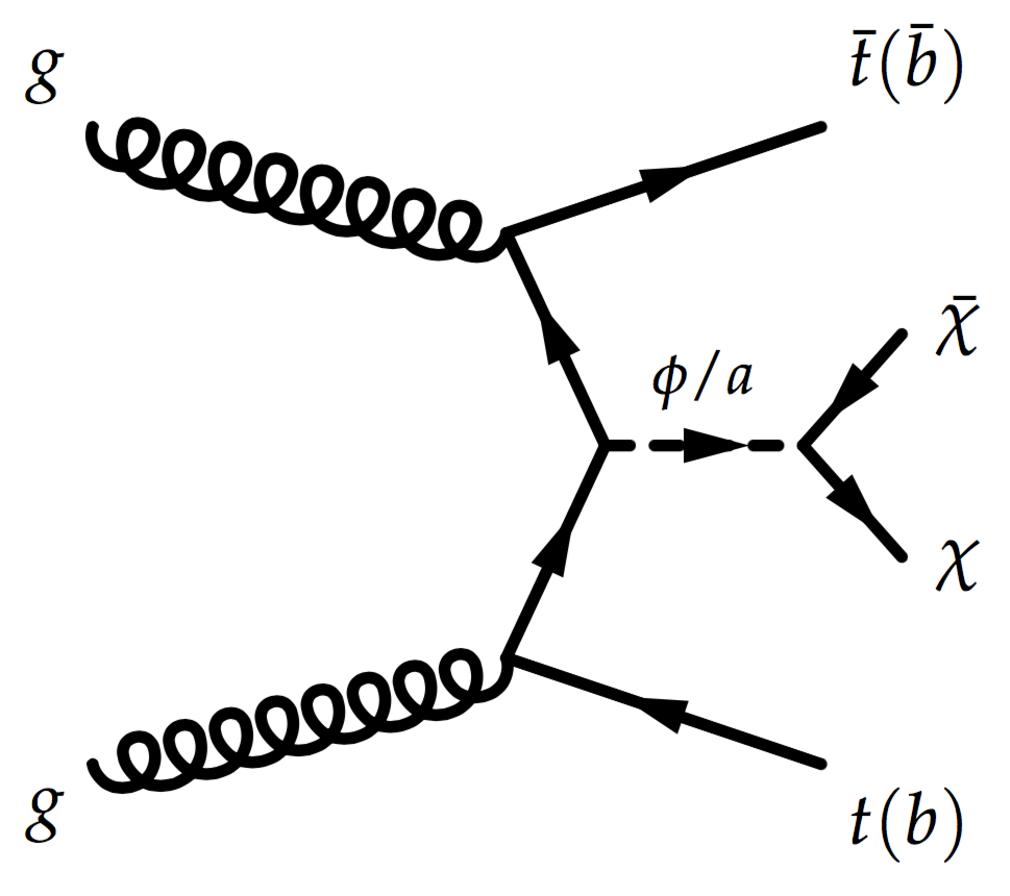
\includegraphics[width=0.5\textwidth]{figures/DMplots/feynman_hf.pdf}}
  \caption{Feynman diagram showing the pair production of Dark Matter particles in association with $t\bar{t}$ or $b\bar{b}$). \cite{Abercrombie:2015wmb}}
  \label{fig:feynman_hf}
\end{figure}


Expected efficiencies and signal yields for nominal, asymmetric and total selection can be found for 3~fb$^{-1}$ in Tables~\ref{tab:dmtt_S},~\ref{tab:dmtt_P}.

\begin{table}[h!]
\small
\centering
\begin{tabular}{l|lllll}
\hline
sample             & $\sigma$ [pb] & Sum Evts       & Evts Sym. Bin & Evts Asym. Bin & Eff  [\%]   \\\hline
Mchi1000\_MPhi1000 & 9.44E-09 & 0      & 0      & 0     & 21.45 \\
\hline
\end{tabular}
\caption{Selected DM+$t\bar{t}$ scalar samples. Given are production cross section, event yields for 3~fb$^{-1 }$ for the various selections and the overall selection efficiency for $g_\textrm{DM}=g_\textrm{SM}=1$ \label{tab:dmtt_S}}
\end{table}

\begin{table}[h!]
\small
\centering
\begin{tabular}{l|lllll}
\hline
sample             & $\sigma$ [pb] & Sum Evts       & Evts Sym. Bin & Evts Asym. Bin & Eff  [\%]   \\\hline
Mchi1000\_MPhi1000 & 3.93E-08 & 0     & 0     & 0     & 20.87 \\
\hline
\end{tabular}
\caption{Selected DM+$t\bar{t}$ pseudo-scalar samples. Given are production cross section, event yields for 3~fb$^{-1 }$ for the various selections and the overall selection efficiency for $g_\textrm{DM}=g_\textrm{SM}=1$ \label{tab:dmtt_P}}
\end{table}

\clearpage
\subsubsection{Projected sensitivities}

Expected signal strength $\mu$ for simplified dark matter models using scalar and pseudo-scalar couplings are calculated for 3~fb$^{-1 }$ and 10 fb$^{-1 }$. Table~\ref{tab:dmtt_S_R_values} lists these
values for the DM and mediator masses $m_\textrm{DM}$, $m_\Phi$ recommended by the DM forum for the scalar operator. The corresponding results for the pseudo-scalar couplings are given in Table~\ref{tab:dmtt_P_R_values}. 

\begin{table}
  \small
  \centering
\begin{minipage}{.45\textwidth}{
  \begin{tabular}{lll}
    \hline                      
    $m_\textrm{DM}$ & $m_\Phi$  & R 3~fb$^{-1}$  \\ \hline
    1       & 10      & 0.32    & 0.18 \\ \hline
  \end{tabular}
  \caption{Projected  upper limits on signal strength $\mu$ for 3~fb$^{-1}$  for the scalar  DM+$t\bar{t}$ models. \label{tab:dmtt_S_R_values}}
}\end{minipage}%\end{table}
\hfill
%\begin{table}[h!]
%  \centering
\begin{minipage}{.45\textwidth}{
  \begin{tabular}{lll}
    \hline                      
    $m_\textrm{DM}$ & $m_\Phi$  & R 3~fb$^{-1}$  \\ \hline
    1       & 10      & 1.8     & 1.0 \\ \hline
  \end{tabular}
  \caption{Projected  upper limits on signal strength $\mu$ for 3~fb$^{-1}$  for the pseudo-scalar DM+$t\bar{t}$ models. \label{tab:dmtt_P_R_values}}
}\end{minipage}
\end{table}




\clearpage
Figure~\ref{fig:limits_DMtt_S} shows the expected exclusion contours for  3~fb$^{-1}$ for scalar $DM+t\bar{t}$ models. 

\begin{figure}[h!]
  \centering
  \subfigure{\includegraphics[width=0.7\textwidth]{figures/DMplots/bla.pdf}}
  \caption{\label{fig:limits_DMtt_S} Expected exclusion contours at 95\% CL for 3\fbinv and 10\fbinv for  scalar $DM+t\bar{t}$ models. }
\end{figure}


